\eat{
\begin{figure*}
    \centering
    \begin{tabular}{ccc}
        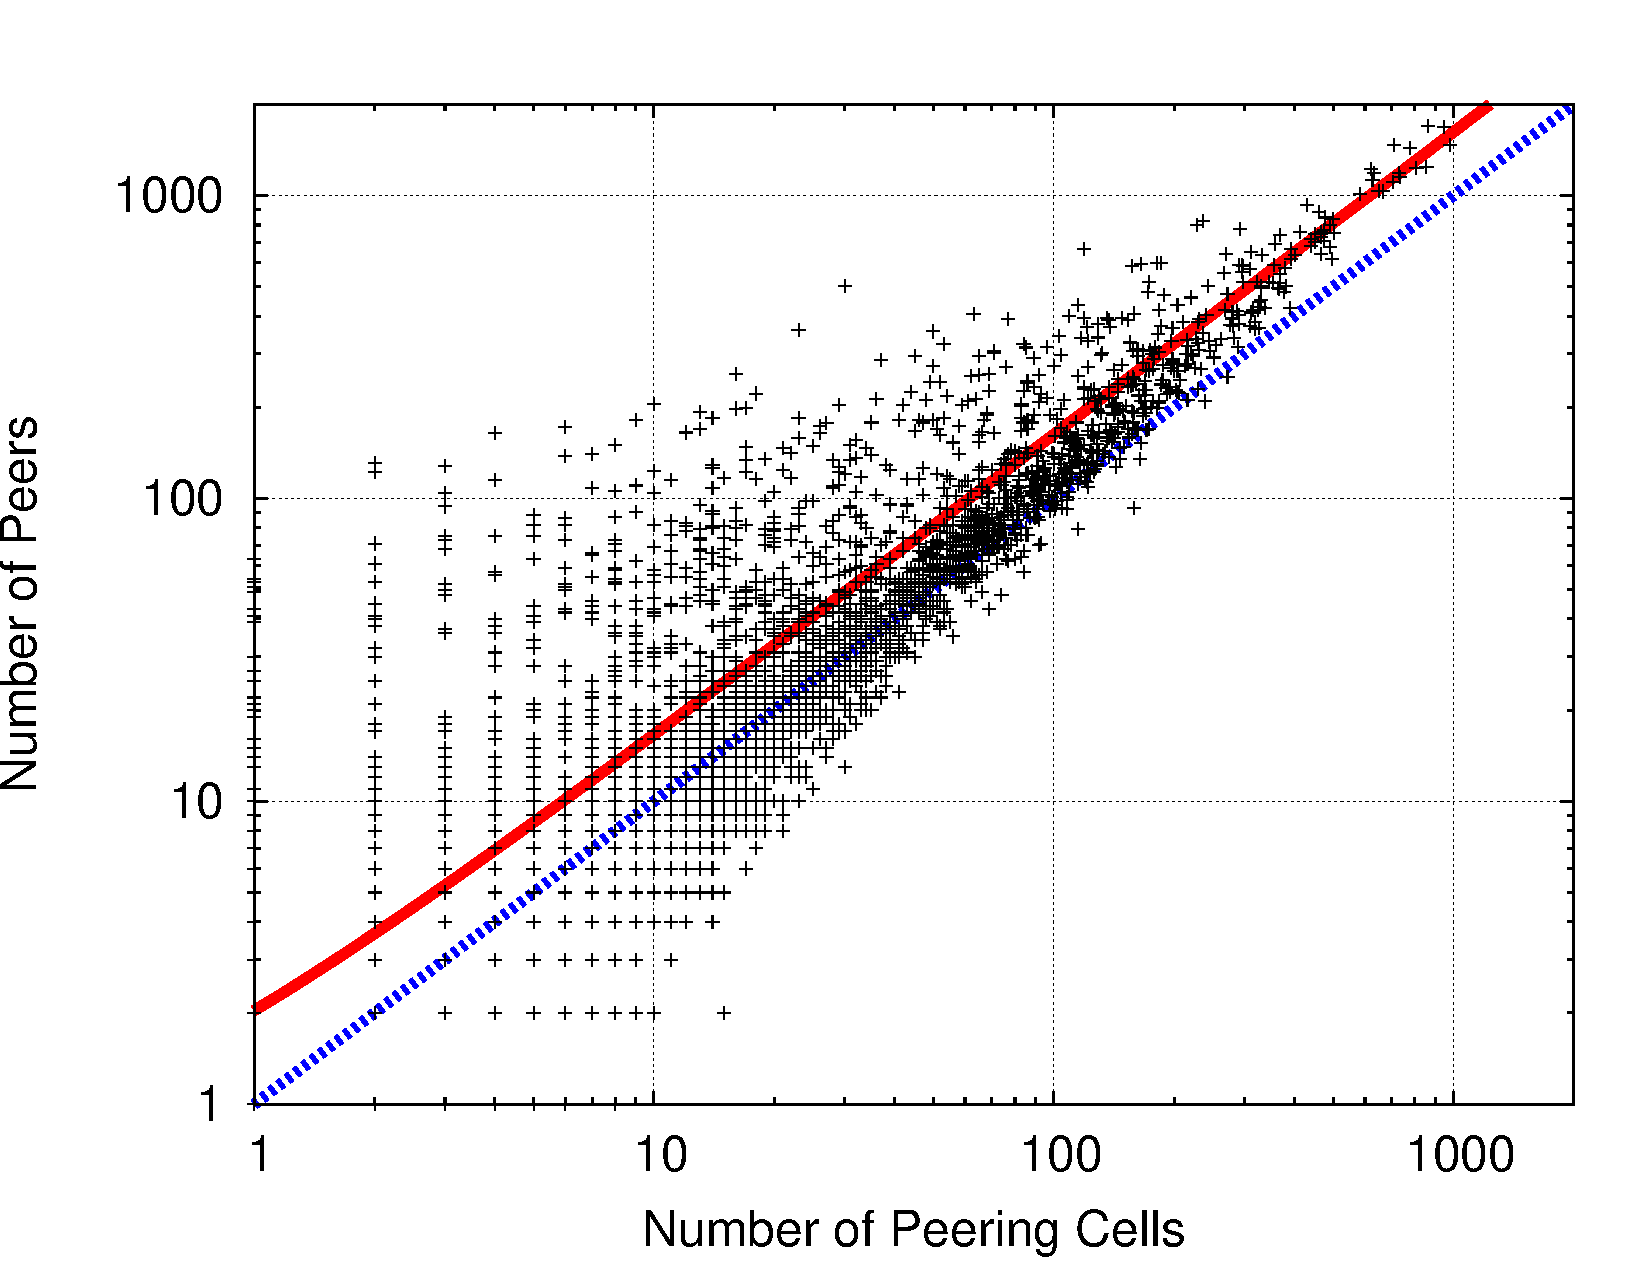
\includegraphics[width=2.2in]{scatter}&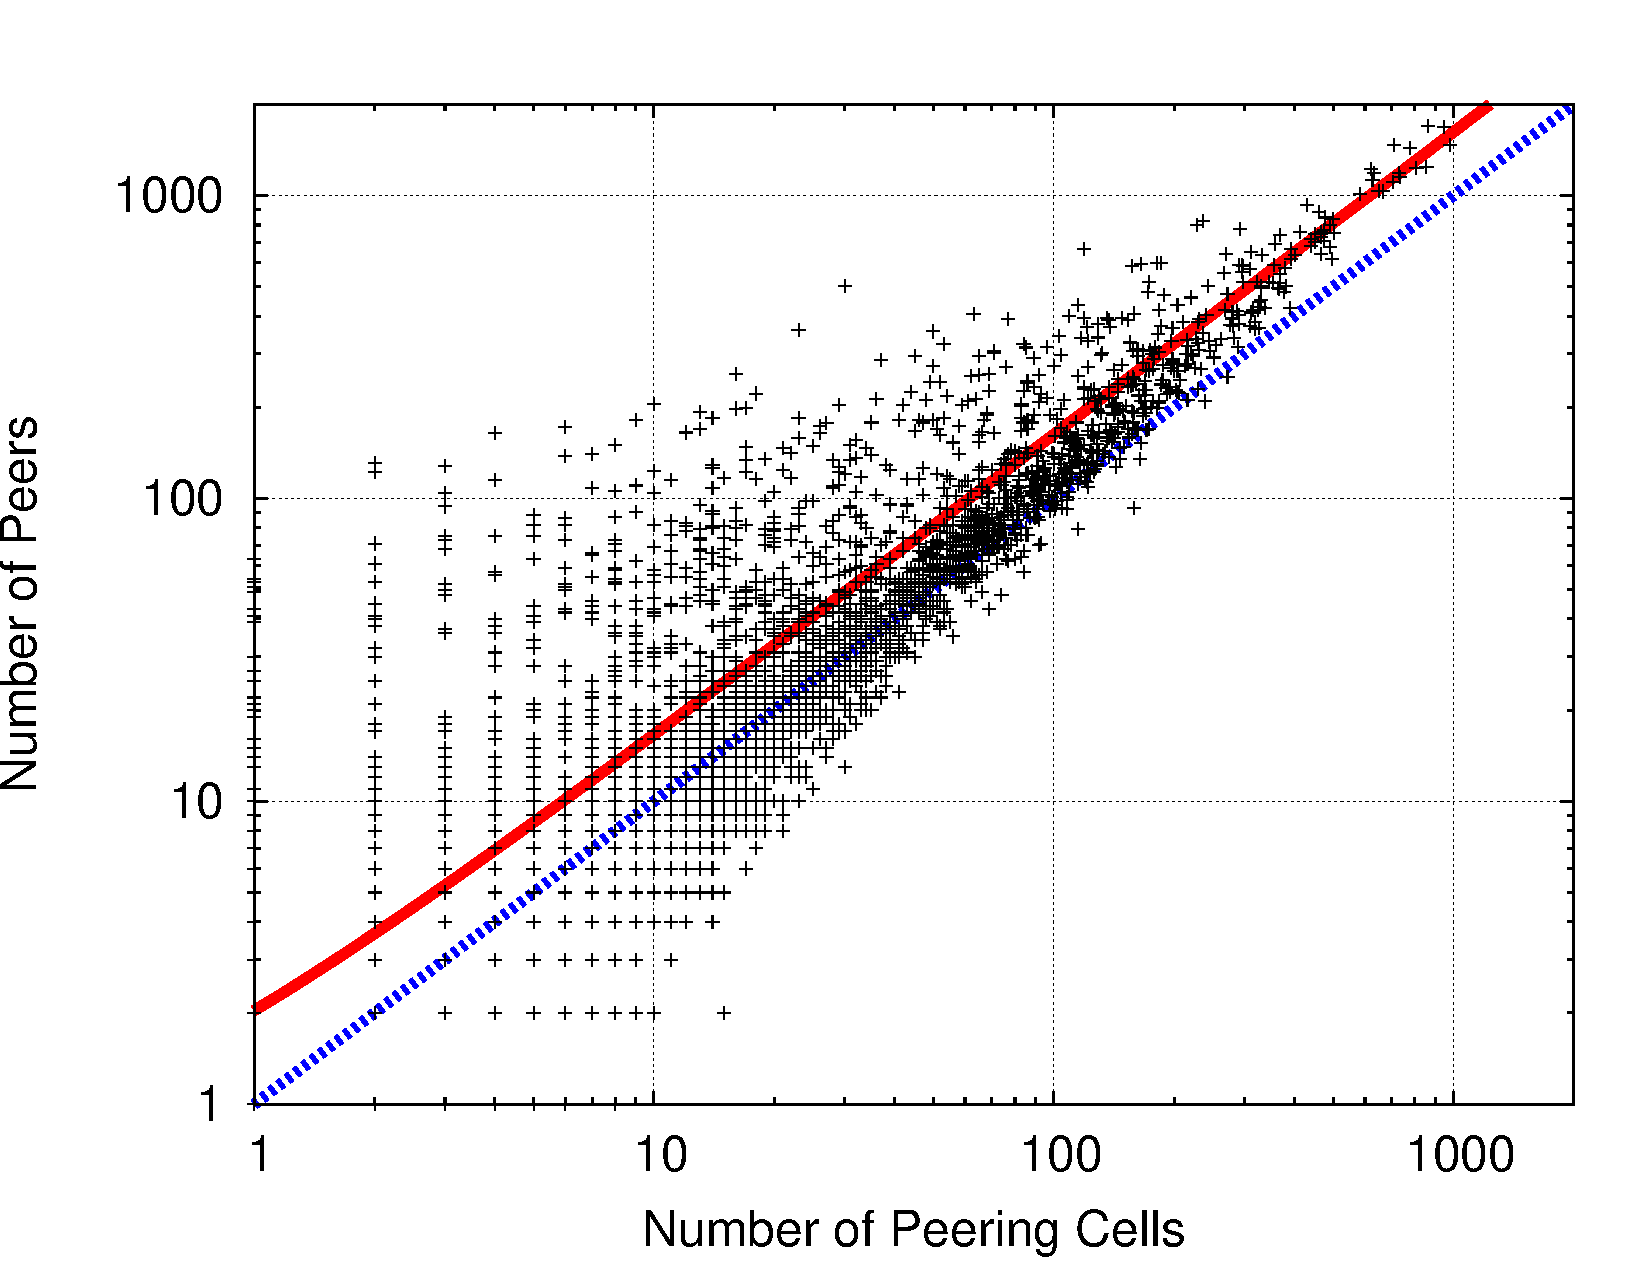
\includegraphics[width=2.2in]{scatter}&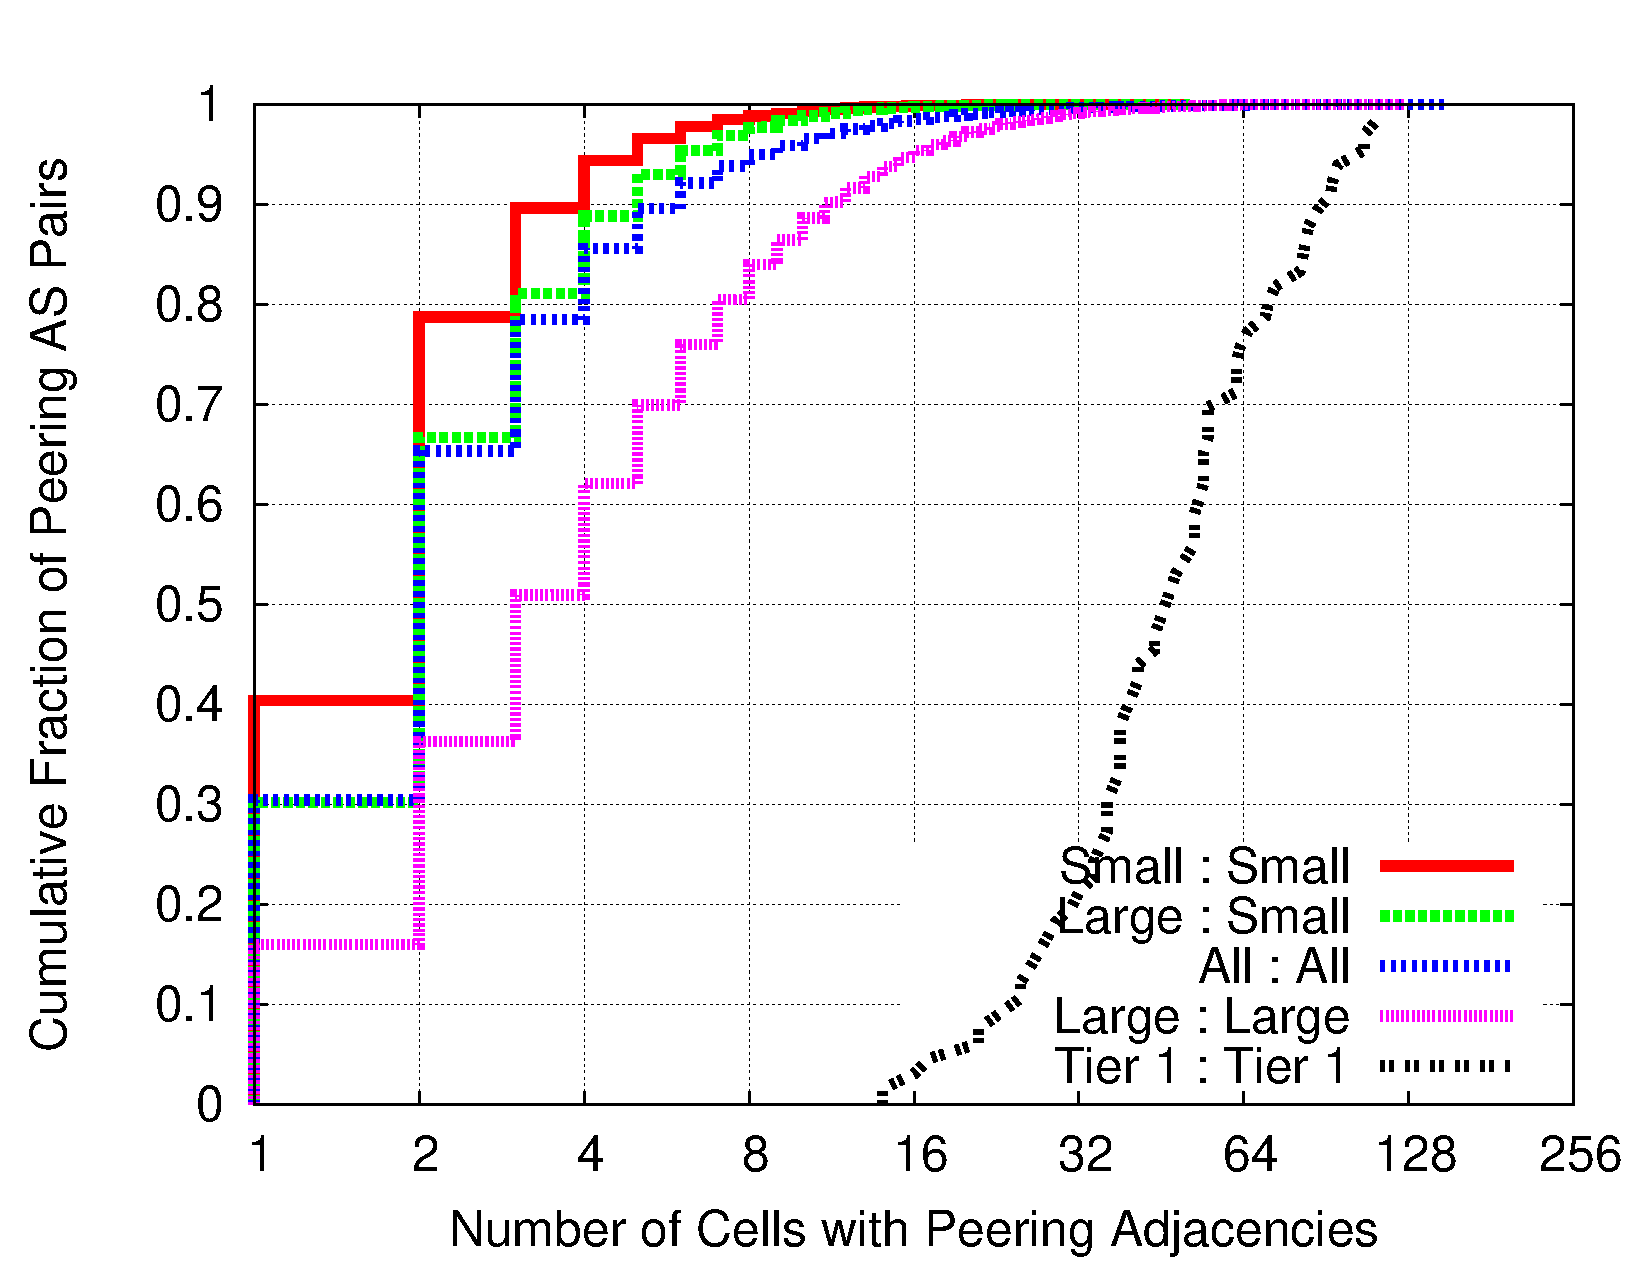
\includegraphics[width=2.2in]{peering}\\
    \end{tabular}
\end{figure*}    
}

    \begin{figure}[tb]
\centering
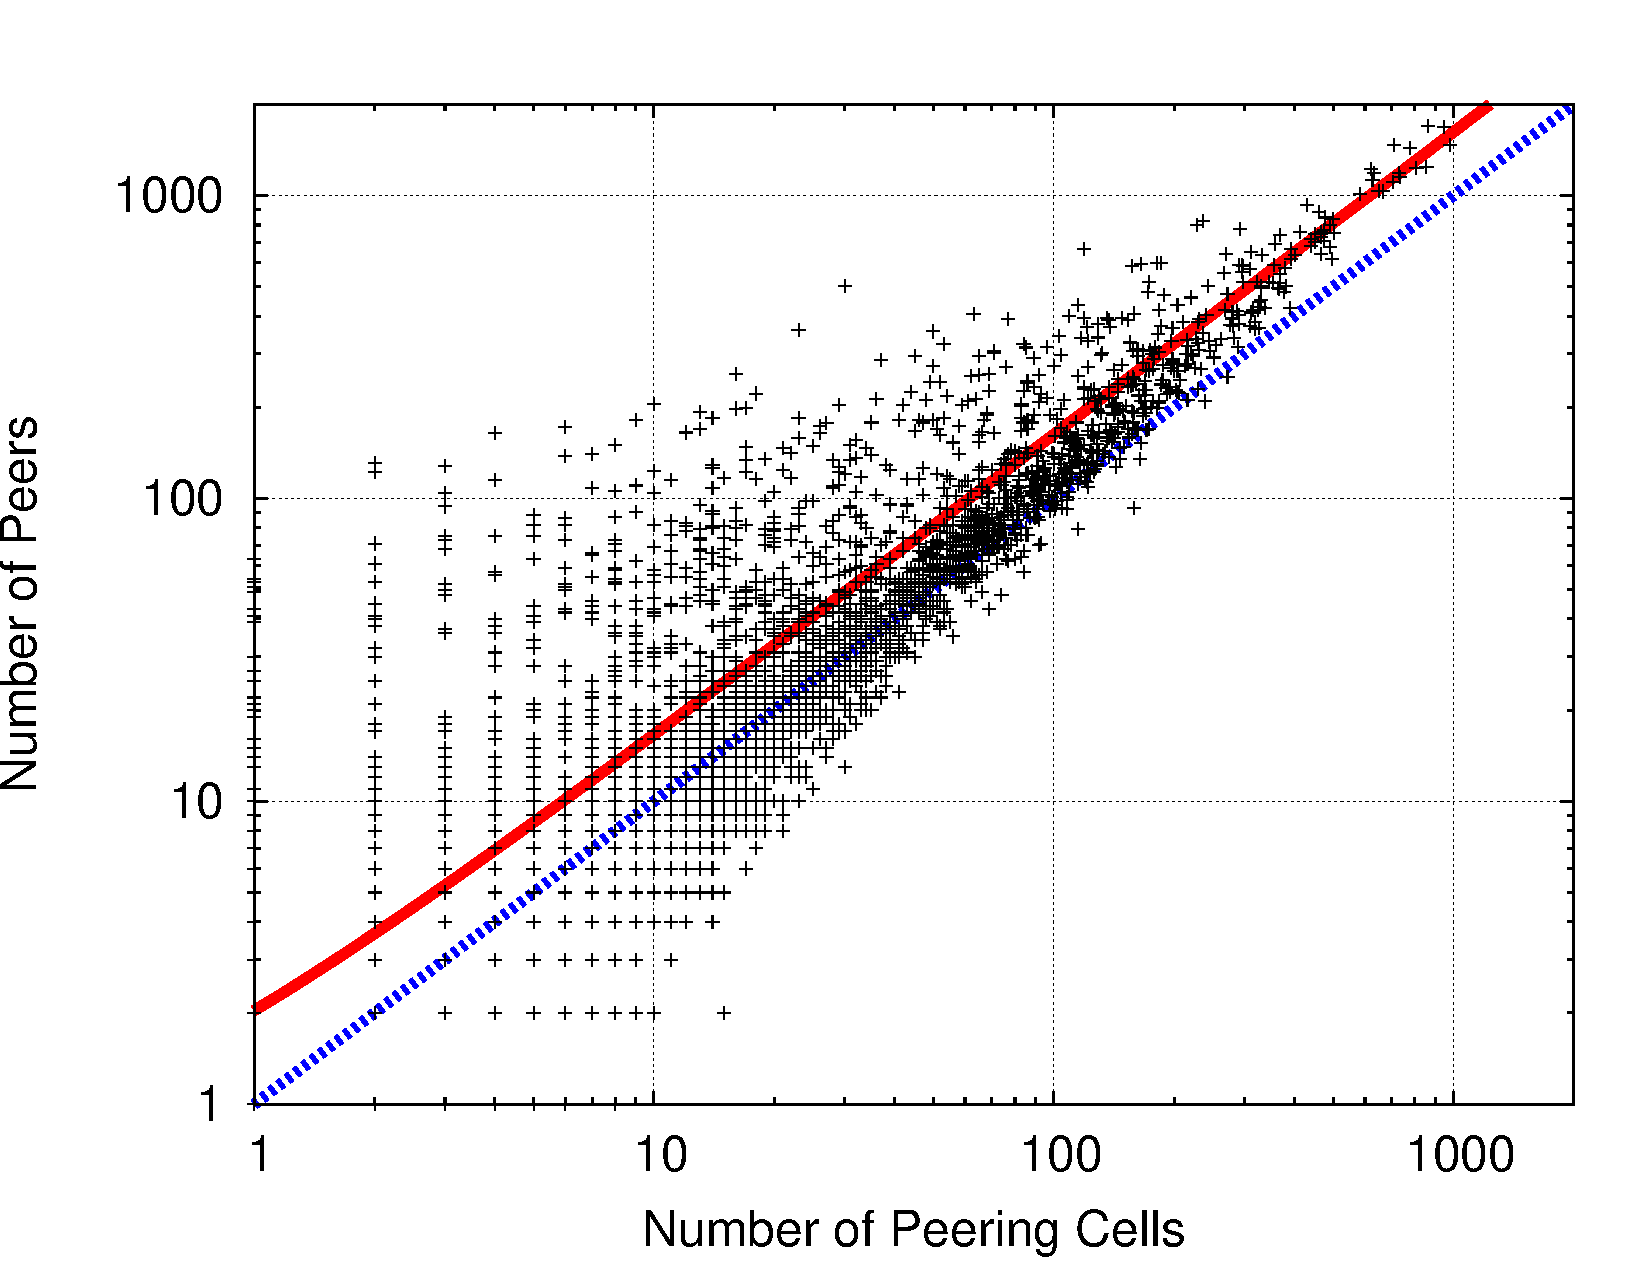
\includegraphics[width=3.25in]{scatter}
\caption[]{\label{fig:scatter} Scatter plot of observed peers to cells with peering adjacencies. Each point represents an AS which has peerings in $x$ cells of the globe, with $y$ total peers. A linear regression (shown, upperline) predicts the ratio of cells to peers to be .625 in the average case. The lower line shows a 1:1 ratio.} 
\end{figure}

\begin{figure}[tb]
\centering
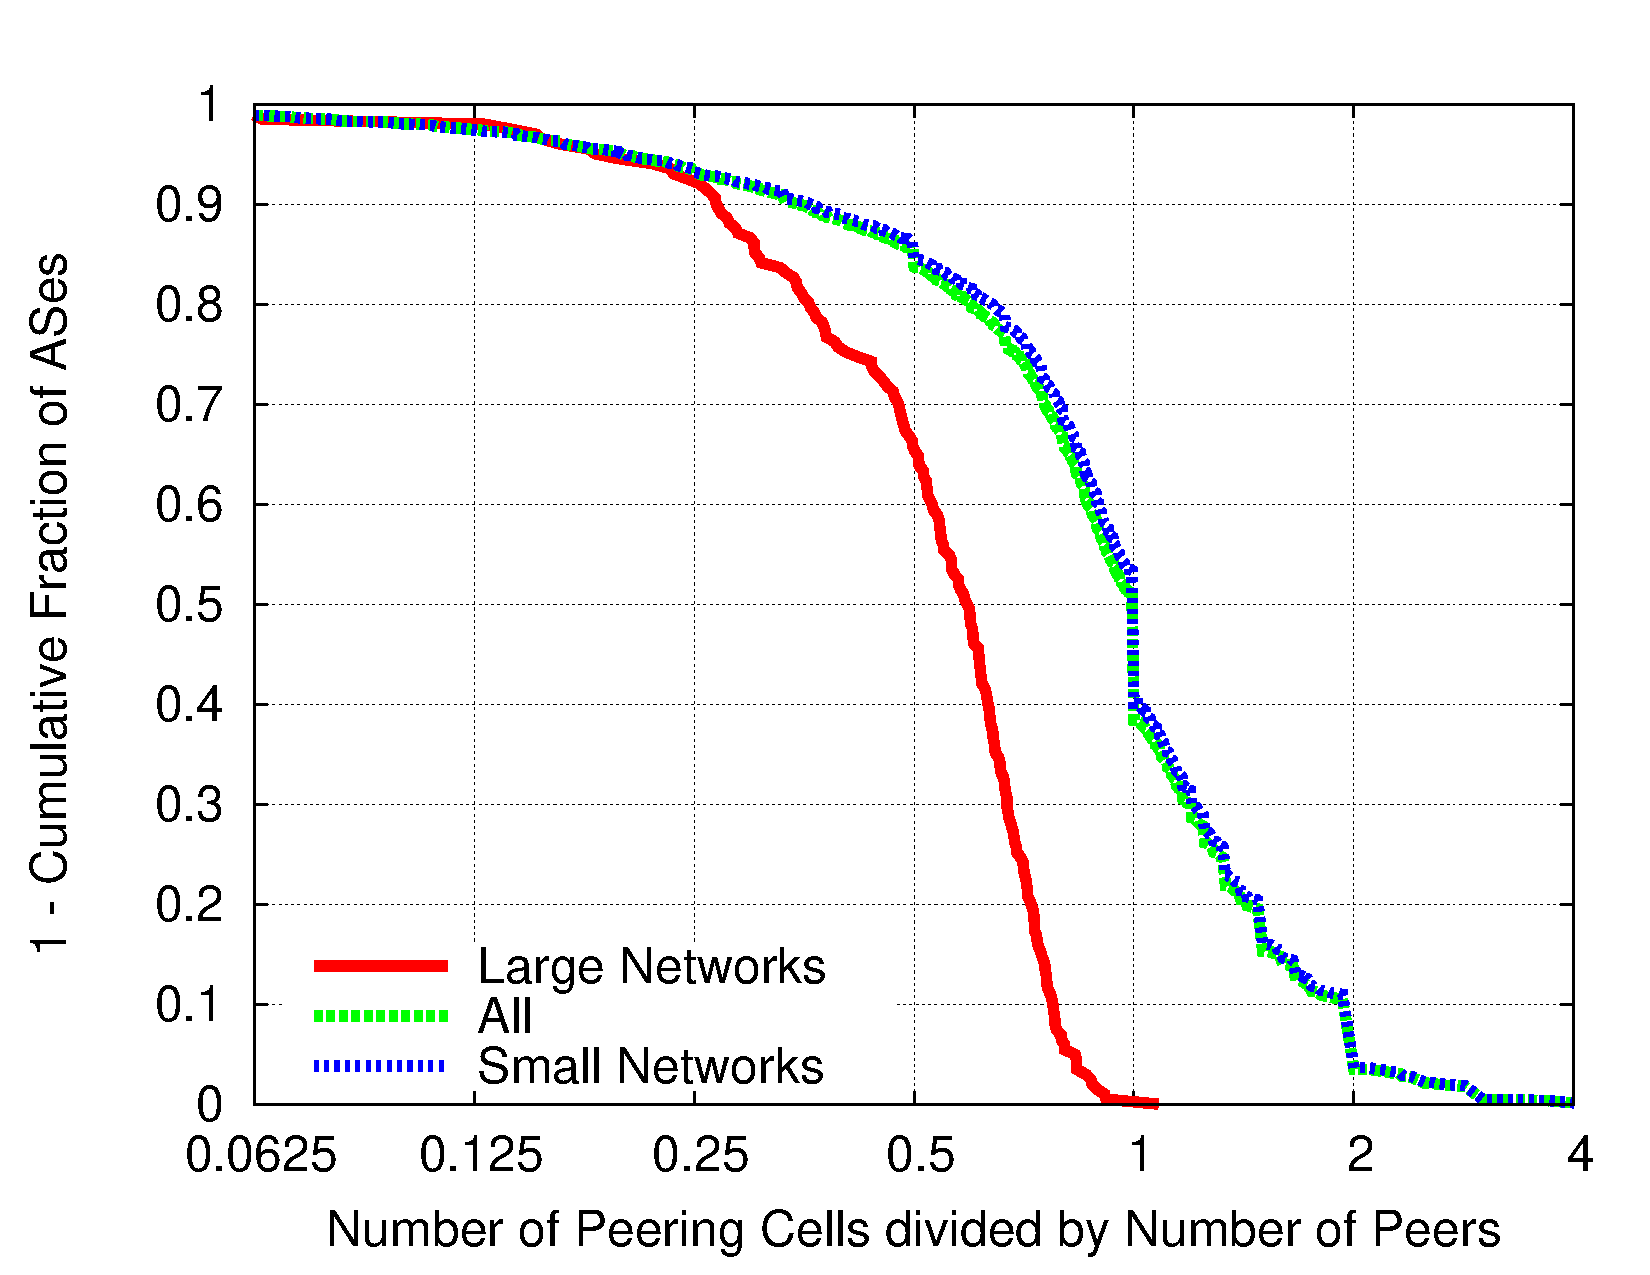
\includegraphics[width=3.25in]{ratio}
\caption[]{\label{fig:ratio} Cumulative distribution of geographic redundancy ratio: the number of cells a network peers in divided by the number of peers it has.} 
\end{figure}




 


    We now provide some basic observations about our data: the number of regions ASes peer in, and how many redundant peering locations ASes maintain per peering relationship.
    We note that, while 84\% of networks are `stub' networks that provide transit to no one, usually with few providers and limited geographic extent, we focus our analysis on networks which provide transit to other networks.
    While the failure of stub networks has no impact on the connectivity graph besides its own disconnectivity, transit networks have entire networks as customers and thus their resilience is important not only for their own connectivity, but that of other networks.

\subsubsection*{Geographic Diversity}
    We first investigate the geographic diversity of peering locations for a single AS, with attention to how the number of peering locations scales with number of neighbors a network has.
    Figure~\ref{fig:scatter} illustrates the range of values for both number of peers ($y$-axis) and number of cells in which the network connects to its peers ($x$-axis).
    We see the number of observed peers range from one (\ie{} the network's provider, since we removed stub ASes from the dataset) to well over 1000 for what must be Tier-1 networks.
    The number of peering locations ranges from one - even for networks with some tens of peers - to hundreds.
    The number of peering locations scales linearly with the number of peers; a linear regression (shown) plots the ratio  at 3 peers to one peering point. 
    However, there are a large number of ASes and the scatterplot is wide around the linear plot for smaller numbers of peers and locations.


    To better investigate this ratio, Figure~\ref{fig:ratio} shows a CCDF of the number of peering cells to number of peers for Tier 1 networks, Large networks (more than 250 peers), Small networks (less than 250 peers), and All networks. 
    Thus, a given $(x,y)$ coordinate means that $y$ fraction of of networks had a ratio larger than $x$ peers for every peering point.
    Here we observe that the average large network has a ratio of .653, while the average small network has a ratio of 1.
    This is because large networks often peer with multiple small networks with whom they only peer in a small fraction of their peering points, while smaller networks often peer with more widespread providers and in a more limited number of locations.
    \justine{This is pure bullshit. I am not sure why and we should - LATER - take time to investigate these graphs.}

\subsubsection*{Peering Redundancy}
    Networks not only maintain multiple peering relationships in multiple locations, but have redundant peering connections in different regions with the same peers.
    In Figure~\ref{fig:peering_redundancy} we plot a CDF of the number of peering cells for AS peering relationships, separating peering relationships between Tier-1 networks, Large (more than 250 peers) networks, and Small networks (less than 250 peers).
    For this graph, an $(x,y)$ point means that $y$ fraction of peering AS pairs connect to each other in less than or equal to $x$ cells on the geodesic globe.

    Since each Tier-1 network forms a large portion of the global backbone, it is no surprise that one pair peers in almost a hundred places, and the least well-connected pair of Tier-1 networks peers in some 14 places.
    Even small (less than 250 peers) networks are typically redundantly connected. 
    While 40\% of peering pairs where both networks are small networks occur in only one cell, the average pair peers in two cells and 20\% peer in three or more cells. 

    Because most transit-providing networks peer with other transit providing networks redundantly, this greatly diminishes the likelihood of a regional disaster or outage disconnecting two transit-providing networks.
    While such a disaster may have impact on intradomain connectivity, interdomain connections are at least once redundant for small transit networks, and tens of times over in the case of the largest networks.

\begin{figure}[tb]
\centering
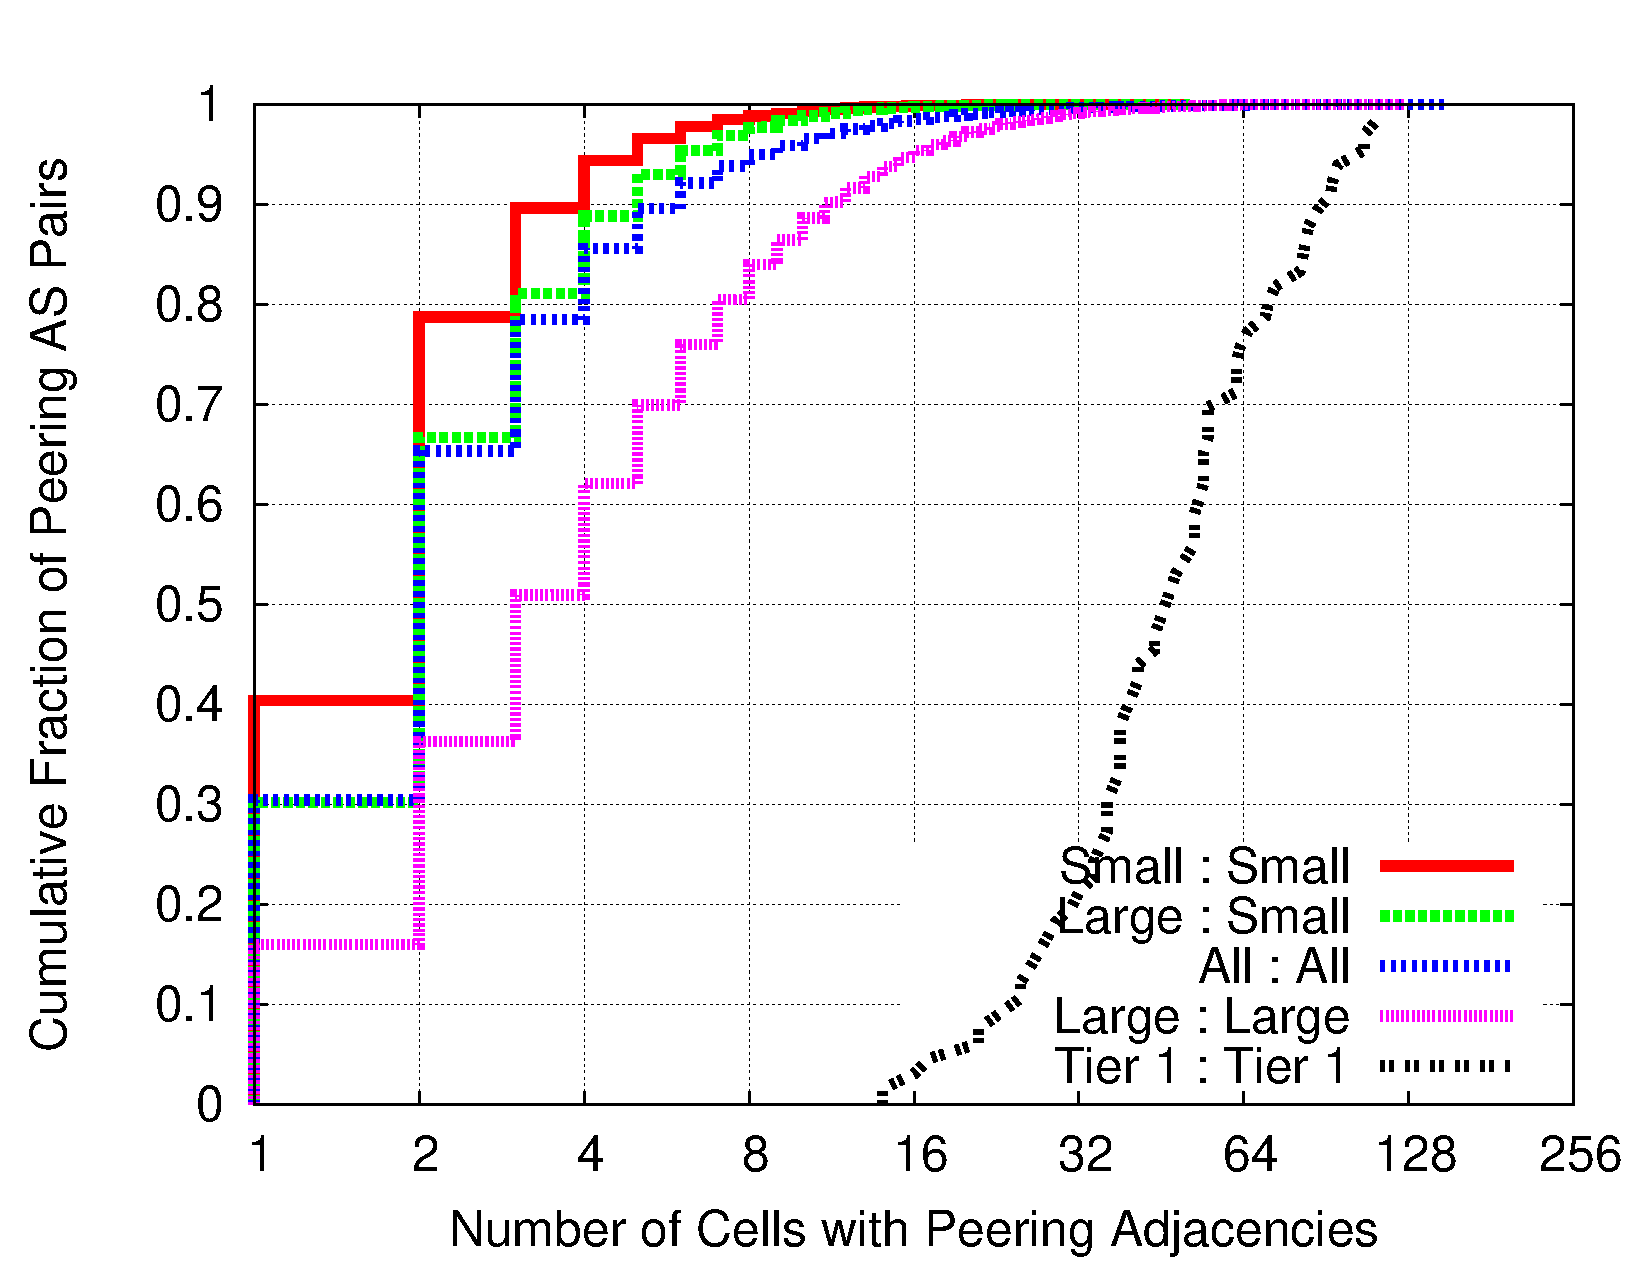
\includegraphics[width=3.25in]{peering}
\caption[]{\label{fig:peering_redundancy} Cumulative Distribution of AS Pairs with redundant regional connectivity. Only 16\% of peerings between large networks occur in only one cell, and 40\% of peerings between small networks occur in only one cell.} 
\end{figure}

